% Copyright Javier Sánchez-Monedero.
% Please report bugs and suggestions to (jsanchezm at uco.es)
%
% This document is released under a Creative Commons Licence 
% CC-BY-SA (http://creativecommons.org/licenses/by-sa/3.0/) 
%
% BASIC INSTRUCTIONS: 
% 1. Load and set up proper language packages
% 2. Complete the paper data commands
% 3. Use commands \rcomment and \newtext as shown in the example

\documentclass[a4paper,twoside,10pt]{reviewresponse}

% 1. Load and set up proper language packages
%\usepackage[utf8x]{inputenc}
\usepackage{newtxtext}
\usepackage{newtxmath}
\usepackage[latin9]{inputenc}
\usepackage[T1]{fontenc}
\usepackage[english]{babel}
\usepackage{natbib}
\usepackage{float}
\usepackage{multirow}
\usepackage{booktabs} % For formal tables

% 2. Complete the paper data
\newcommand{\myAuthors}{Chaiyong Ragkhitwetsagul,~Jens Krinke,~Matheus Paixao,~Giuseppe Bianco,~Rocco Oliveto}
\newcommand{\myAuthorsShort}{Ragkhitwetsagul et. al}
\newcommand{\myEmail}{{chaiyong.ragkhitwetsagul.14,j.krinke,matheus.paixao.14}@ucl.ac.uk, giuseppebianco92@gmail.com, rocco.oliveto@unimol.it}
%\newcommand{\mySecEmail}{}
\newcommand{\myTitle}{Cover Letter for the Reviewers of the Paper \\ ``Toxic Code Snippets on Stack Overflow''}
\newcommand{\myShortTitle}{Cover Letter}
\newcommand{\myJournal}{IEEE TRANSACTIONS ON SOFTWARE ENGINEERING}
\newcommand{\myDept}{University College London (UK), University of Molise (Italy)}
%%%%%%%%%%%%%%%%%%%%%%%%%%%%%%%%%%%%%%%%%%%%%%%%%%%%%%%%%%%%%%%%%%%%%%%%%%


%\usepackage[linktoc=all]{hyperref}
\usepackage[linktoc=all,bookmarks,bookmarksopen=true,bookmarksnumbered=true]{hyperref}

\hypersetup{
pdfauthor = {\myAuthorsShort},
pdftitle = {\myTitle},
pdfsubject = {\myJournal\xspace},
colorlinks = true,
linkcolor=blue,          % color of internal links
citecolor=black!70!green,        % color of links to bibliography
filecolor=magenta,      % color of file links
urlcolor=black           % color of external links
}

\newcommand\FIXME[1]{{\color{red}\textbf{FIXME: #1}}}

\begin{document}

\thispagestyle{plain}

\begin{center}
 {\LARGE\myTitle} \vspace{0.3cm} \\
 {\large\myJournal} \vspace{0.3cm} \\
 \today \vspace{0.3cm} \\
 \myAuthors \\
 \url{\myEmail} \\
 %\url{\mySecEmail} 
 \vspace{0.3cm} 
 \myDept \vspace{1cm}
\end{center}

%\tableofcontents

%\begin{abstract}
This paper is a journal-first submission to Transactions on Software
Engineering. This is a re-submission of the previous submission
no.~TSE-2017-11-0335 and we would like to thank the anonymous Reviewers for
taking their time to carefully read our paper. With their useful and
constructive reviews, we substantially improved the work by adding three major
improvements as listed below to our previous submission and minor improvements
as discussed later in this letter:

\textbf{1. A study of toxic code snippets on GitHub:}~To provide an evidence
that toxic code snippets are actually reused in software projects and strengthen
the motivation, we performed a large-scale analysis of clones between the
discovered 100 outdated code snippets on Stack Overflow and 130,703 GitHub
projects using a clone detection tool and a manual validation.

\textbf{2. Analysis of tools' parameter settings:}~We mitigated the threats to
validity due to parameter settings of the clone detection tools and the clone
merging technique by performing a comparison of different tools' parameter
settings.

\textbf{3. Extended analysis of online code clones:}~We performed more analyses
on the 2,289 online code clones and 100 outdated code snippets. For example,
we analysed the size and age of the clones, and summarised the six intents that
made the clones outdated.

\textbf{4. Revisions to the overall discussion:}~We substantially expanded the
overall discussion to include (1) a discussion of toxicity of outdated and
license-incompatible clones on Stack Overflow, and (2) more detailed discussion
of how to implement the tools or approaches proposed in the preventive and
detective measures.

We also tried our best to address all the comments from the reviewers. Every
comment led to an improvement(s) on this submission and we discuss them in order as shown in the
next sections.

\clearpage

\section{Reviewer 1}

\rcomment{
Regarding this statement: \textit{``It is probably more important than studying the effects of reusing Stack Overflow code snippets because it gives insights to the root cause of the problem and lays a foundation to an automatic technique to detect and report toxic code snippets on Stack Overflow to developers in the future.''}

While~\cite{An2017} do suggest that copying from Stack Overflow to software projects occurs (and results in license violations), they do not establish that code snippets from Stack Overflow \textit{``go viral''} and end up distributed widely across (open or closed source) software projects. Moreover, while the quote on the first page implies that developers often \textit{``mindlessly''} reuse code snippets from Stack Overflow, to the best of my knowledge, this claim is conventional wisdom but not empirically validated. So, it seems to me that the primary interest in toxic code snippets is that may cause widespread harm, but I am missing the evidence that they do so in practice. Even assuming that code snippets from Stack Overflow are distributed mindlessly and widely, I wonder how many code snippets on Stack Overflow are toxic, the extent to which they are reused without modification (or with only minor adaptation), what kinds of projects they end up in (i.e., a popular project from Microsoft or Apache vs. a hobby project by a single developer vs. a student solution to an assignment), and ultimately, how much damage can we expect them to cause. In the end, I agree that it is better to detect and report toxic code snippets than to not do so, but I am not sure how big of a problem is solved by doing so. As such, I disagree that it is \textit{``probably more important''} to find the toxic code snippets than to understand their effects. Instead, I think that understanding their effects (on software projects rather than on the quality of the Stack Overflow platform) is necessary to appreciate the value in finding them.
}

We would like to thank the reviewer for the comments.~We agree with the suggestion and we made the following changes to the paper:

\begin{enumerate}
	\item We understand the concern of finding real evidence to support that code snippets on Stack Overflow do appear in software projects. Hence, we have performed a study of code clone detection between our 100 reported outdated code snippets on Stack Overflow and 131,703 GitHub projects ranging from 29,465 stars to 1 star. We selected SourcererCC with 80\% similarity for this experiment because it could scale to a large-scale data set, while Simian could not. We found 102 cloned candidates appearing in 68 GitHub projects and manually investigated all of them. As shown in the table below, out of the 102 cloned snippets, there were 13 cloned snippets that matched with themselves because some of the Qualitas projects also appear on GitHub. For other projects besides the Qualitas projects, there were 47 cloned snippets that were exactly the same as the outdated code snippets and 42 cloned snippets that were not exactly the same (e.g.~they contained additional code modifications made by the projects' developers or they were copied from another source with a slightly different code). 
	
	\begin{table}[H]
		\centering
%		\caption{Clones of the 100 Stack Overflow outdated code snippets in 131,703 GitHub projects}
		\label{tab:outdated_github}
		\begin{tabular}{lr}
			\toprule
			Clones & Amount \\
			\midrule
			\textit{Found in Qualitas GitHub repos} & 13 \\
			\midrule
			\textit{Found in other project repos} & \\
			Exact copy (outdated) & 47 \\
			Non-exact copy & 32 \\
			\midrule
			Total & 102 \\
			\bottomrule
		\end{tabular}
	\end{table}

	Among the exact-copy of 47 outdated cloned snippets, there were only two cloned snippets that gave attributions to Stack Overflow. However, the attributions pointed to different posts than the ones we found, but containing the same code in the answers. The other 32 cloned snippets were very likely to be a file-level clone from its respective original project (e.g. JFreeChart, JUnit, Log4J, Hadoop) based on their license header and the Javadoc comments. Lastly, the remaining 13 cloned snippets did not have any hints or evidence of copying.
	
	Interestingly, we discovered that the buggy version of the \texttt{humanReadableInt()} method from Hadoop appears in two popular Java projects: deeplearning4j (8,830 stars and 4,223 forks) and Apache Hive (1,854 stars and 1,946 forks). Due to the lack of evidence, we could not conclude how this method, which is exactly the same as the toxic code snippet we found on Stack Overflow, appear in the two projects. It is possible that the developers retrieved them from Stack Overflow, other websites, or from Hadoop code base directly.  
	Nevertheless, we decided to report the developers of the two projects regarding the issue. We created a bug report for each project (deeplearning4j \#4694\footnote{deeplearning4j bug report: \url{https://github.com/deeplearning4j/deeplearning4j/issues/4692}} and HIVE-18929\footnote{Apache Hive bug report: \url{ https://issues.apache.org/jira/browse/HIVE-18929}}) and communicated with the developers of the projects by describing the problem of race condition in the outdated version of \texttt{humanReadableInt()} method and proposed a fix by using the newest version of the method in Hadoop. The issue has been fixed in deeplearning4j. The developers of deeplearning4j agreed that the method was problematic and they decided to implement their own fix due to a concern of a potential software licensing conflict caused by copying the fix directly from Hadoop code base. On the other hand, the bug report in Apache Hive is still unfixed.
	
	\item The same study has been done for another type of toxic code snippets on Stack Overflow, license-incompatible code snippets. We detected clones between the 214 code snippets without their original license (86 QS, 78 EX and 50 UD)  and 130,703 GitHub projects using SourcererCC with 80\% similarity threshold. 
	Then, we used the Ninka tool to automatically identify software license from the 7,207 code snippets.
	Opposite to the outdated clones, we discovered many more clones of 7,207 candidate pairs. There were 90 pairs from 10 Qualitas projects on GitHub and 7,117 pairs from 
	2,427 other projects. From the Table \ref{tab:license_github} shown below, the clones were found from highly-starred projects (29,465 to 10 stars) to 1-star projects. 
	
	\begin{table}[H]
		\centering
		\label{tab:license_github}
		\begin{tabular}{l|rr|rrr}
			\toprule
			\multirow{2}{*}{No. of stars} & \multicolumn{2}{c|}{Qualitas} & \multicolumn{3}{c}{Other Projects} \\ \cmidrule{2-6}
			& Projects & Clone Pairs & Projects & Clone Pairs & Same license \\
			\midrule
			29,540 to 10 stars & 8 & 71 & 406 & 1,837 & 193 \\
			9 to 5 stars & 0 & 0 & 275 & 739 & 110 \\
			4 to 1 stars & 2 & 24 & 1,746 & 4,536 & 692 \\
			\midrule
			Total & 10 & 95 & 2,427 & 7,112 & 995 \\
			\bottomrule
		\end{tabular}
		\caption{Clones of the 214 Stack Overflow missing-license code snippets in 131,703 GitHub projects}
	\end{table}
	
	\item With the finding above, we show that the clones of Stack Overflow toxic code fragments do occur in several open source software projects on GitHub. However, we could not establish a strong evidence that the toxic code snippets were originated from Stack Overflow due to lack of supporting information. Hence, we softened our claim by changing the statement ``\textit{It is probably more important than studying the effects of reusing Stack Overflow code snippets ...}'' to ```\textit{It is \textbf{equally} important to studying the effects of reusing Stack Overflow code snippets ...}''.
	We also updated the Overall Discussion section to reflect the findings that (1) there is only a small number of toxic code snippets from outdated code that are found in GitHub projects, (2) there is a large number of toxic code snippets from missing license that are found in GitHub projects. %Moreover, the direction of copying is also unclear. The clones could come from Stack Overflow, the original project repositories, or other places. 
\end{enumerate}

\rcomment{
	I think that the survey evidence is compelling. But I am missing the awareness of Stack Overflow questioners or information-seekers to toxic code snippets. I wonder: how skeptical are developers when considering code snippets on Stack Overflow, how often do developers use code snippets directly, and how often do developers use clues such as \textit{``A quick google search returned me this from Appache hadoop project. Copying from there:''} to seek out the latest version of the information provided in the answer. The survey responses described in Section 3.5.3 suggest that there are questioners/information-seekers that are aware of toxic code snippets (as they are reporting them to the answerers), and there is evidence that the Stack Overflow community is aware of the need to retire outdated information and of the many concerns related to software licensing, as these issues are discussed on meta.stackoverflow.com. So, again, I wonder about the impact of toxic code snippets on actual software projects.
}

We partially address this comment in the previous answer by performing an empirical study of code cloning between Stack Overflow toxic code snippets and GitHub projects. Furthermore, we also improved the paper on the aspect of the awareness of information-seekers to toxic code snippets on Stack Overflow by including the results from another survey of Stack Overflow visitors (i.e.~information seekers). This survey of the Stack Overflow visitors was performed during the same time as the Stack Overflow answerers (25 July 2017 to 25 September 2017) and the full results are reported in our technical report~\citep{Ragkhitwetsagul_RN2017}. We did not include the results in the previous version of the paper due to a smaller sample size compared to the answerers survey. However, we did find some interesting results so we have included them into this version and discussed the key findings in~RQ1. The brief summary of the visitor survey is as follows.

\textbf{Stack Overflow visitors' survey}

We surveyed 87 Stack Overflow visitors (visit the site and reuse code from Stack Overflow at least once) via five channels: social media post (Facebook),
\textsf{blognone.com}, a popular technology news and media community in Thailand, the University of Molise in Italy where the third author works, \texttt{comp.lang.java.programmer} group and the Software Engineering
Facebook page.

The visitors survey confirms the findings from the previous studies that Stack
Overflow code snippets can be problematic~\citep{Zhang2018,Acar2016,An2017}. Sixty-six
percent of the visitors experienced a problem from reusing Stack Overflow code
snippets ranging from incorrect solutions, outdated solutions, mismatched
solutions, to buggy code. Although they are aware of the problems, half of them
(56\%) never reports back to the Stack Overflow discussions. On the other hand,
the visitors rarely give attributions to Stack Overflow when they reuse code
snippets from the website, similar to the findings reported
by~\cite{Baltes2017}. The visitors are generally not aware of the CC BY-SA 3.0
license, and more than half of them never check for license compatibility when
reusing Stack Overflow code snippets. 
Sixty-nine Stack Overflow visitors (79\%) who adopted code from Stack Overflow never 
check if the code snippet originated from a different source (e.g. an open source project) 
with an incompatible license to their projects.
Moreover, we also found that 9\% of the participants
encountered legal issues by copying code from Stack Overflow. To the best of our
knowledge, a study of legal problems from reusing Stack Overflow code snippets
has never been done before and will be our future work.

The full detail can be found in the RQ1 result section in the paper.

\rcomment{
	The \textbf{Overall Discussion} section is not commensurate with the quality and breadth of the empirical study. The proposed preventative measure is actually two measures: a policy change and an IDE plugin. While an IDE plugin would provide early detection (and possible prevention) of license violations, the exact mechanics are not clear based on the description. Further, companies (and perhaps major open source projects?) use auditing platforms/services to detect such violations. Regarding the detective measure, I do not think that the paper establishes that a system to detect outdated code snippets on Stack Overflow is needed (but rather it establishes that outdated code snippets exist on Stack Overflow). Further, not all outdated code snippets are bad. For instance, a code snippet may show a solution using an older version of an API, and that older version may still be used in production. So, the definition of outdated would need to be a bit more nuanced to be used in an automated system for flagging or updating old Stack Overflow posts.
}

Thanks for the suggestion.~We rewrote the Overall Discussion section to reflect yours and Reviewer 3's comments. The changes include:

\begin{enumerate}
	\item We added a discussion of toxicity of outdated and license-incompatible clones on Stack Overflow. Although we found some harmful outdated clones, we could not find evidence that they are widely reused in open source projects on GitHub. Thus, outdated code snippets may not be so harmful to reuse. On the other hand, the problem of license incompatibility caused by missing original license in Stack Overflow code snippets can cause more damage than outdated code. Different legal system and different interpretation of fair-use concept and de minimis (i.e.~the minimal lines of code allowed to be copied without violating copyright) in each country can result in a legal case in one country becoming illegal in another country. 
	
	\item We performed a study of two open source software auditing
	platforms/services:~BlackDuck
	Software\footnote{https://www.blackducksoftware.com} and
	nexB\footnote{https://www.nexb.com}. For BlackDuck Software, we found from their
	report~\cite{CORSI2017} that while they check for code copied from open source
	projects including GitHub and Stack Overflow and analyse their license
	compatibility with their customer software, the BlackDuck auditing system will
	treat the code snippets on Stack Overflow as having ``unknown'' license because
	it does not know the original license of Stack Overflow code snippets. For nexB,
	their product does not mention checking of reused source code from Stack
	Overflow. So, our proposed service, which can offer more precise licensing
	information of Stack Overflow code snippets, will be useful as an add-on license
	check for code copying from Stack Overflow. We include this in the Overall Discussion.
	
	\item We improved the Actionable Items to be more precise about the mechanics on how to automate the process of finding online code clones, detecting outdated code, and finding license-incompatible code snippets.
\end{enumerate} 

\rcomment{
Other Comments
While ``Toxic Code Snippets'' is a catchy phrase for the title, I think that online code clones are the dominant topic.}

You are right. We mainly study the online code clones and established their existence. However, we used the term ``toxic code snippets'' in order to emphasise the possible ramifications from online code cloning. 
Moreover, the term code cloning is not well known outside the code cloning community. Code clones are called differently in each research community or in practice, such as duplicated code, copy-and-paste code, code reuse, software similarity or software redundancy. So, we decided not to use the term in the title. 

We also updated the Introduction to state that the dominant topic is about online code clones as follows.

``Although this activity of online code cloning is well-known, there is only a few
empirical studies on the topic~\citep{An2017,Abdalkareem2017,Baltes2017}, especially
the on finding the origins of the clones.
We tackle this challenge of establishing existence of online code clones and
investigate how they occur in this study.''
%Considering your suggestion and another suggestion by Reviewer 2 that the definition of ``toxic code snippets'' is vague, we also tightened the definition of toxic code snippets to be more precise.

\rcomment{
	The introduction states that the erroneous code snippet in post 22262310 has been viewed 259 as of the writing of the paper. But I note that while the question was posted on Mar 7, 14 the answer was posted on Mar 11, 14. I also note that the question has a score of -1. So, I wonder (a) whether the view count is for the answer (i.e., the code snippet) or the post (which existed for a few days before the answer appeared), (b) how many people viewed the question before it was answered, and (c) if the negative score for the question impacts both the number of views and the trust that people place in the answer to a down-voted question.}

That is a fair point and we would like to analyse the statistics as you suggested. 
For (a), the number of views
is for the whole Stack Overflow post but we use it as a proxy of the number of views the accepted answer receives
because the question and the answer of the two motivation examples have a short gap of posting time (within the same day and four days after).
For (b), unfortunately, for our experiment we extracted only the code snippets from the Stack Overflow dumps but not other information. They are the only available data of the January 2016 snapshot we currently have. We checked and found that the latest available Stack Overflow dump already contains different data than the one we used in our study since it is now more than 2 years newer, and will result in incorrect statistics and inconsistent results.
For (c), that is a really interesting idea. However, it is out of the scope of this study and would involve an extensive analysis of the data so we plan to do it in the future work.

 Nevertheless, we have added a footnote to the text in the Introduction to clarify point (a).

\rcomment{
	FYI, since this paper was authored, a Stack Overflow user has posted a comment in response to the answer for post 22262310. The comment highlights the missing line and refers to the relevant HADOOP issue report. Interestingly, the gap between the issue report being resolved (Nov 20, 14) and the comment appearing on Stack Overflow (Oct 31, 17) is nearly three years. I wonder how many views occurred during this gap and whether the addition of the comment mitigates the toxicity of the code snippet.
}

Thank you for the detailed checking of the Stack Overflow post. Interestingly, this is surprising to us as well. The comment in the post 22262310 by Joseph K on 31 October 2017 that highlights the missing line in HADOOP \texttt{compare} method is actually from a student in our class. His name is Joseph Kalash and he is a master student in Machine Learning MsC program at UCL Computer Science department \footnote{Joseph's CV can be found here: \url{https://jkala.sh/cv}}. We assigned a preprint of this paper to students in the COMPGS11 -- Research Seminar in Software Engineering course and had a discussion about the paper on Thu 2 November 2017. Joseph, who was an active Stack Overflow member, was one of the students in the class and he actively participated in the discussion. It seemed like he had seen the Hadoop's toxic code snippet in the paper and decided to post a comment to warn other users.

Nevertheless, since this is a very interesting suggestion. We also performed an investigation of the 100 answers of our reported outdated code snippets on Stack Overflow on 6 May 2018 to see if there is any comment to mitigate or point out the toxicity of the code snippet. We include the result of this investigation in the RQ4. We found that, out of 100 answers containing outdated code snippets, there were 6 answers that had a comment saying the code in the answer is outdated or containing issues (including Joseph's comment). Thus, there is about 6\% of outdated answers that were notified by the Stack Overflow users based on our analysed data. None of the 6 answers change their outdated code, but the comments themselves may help to warn other Stack Overflow users. We added this discussion in the RQ4.

\rcomment{
\begin{enumerate}
	\item Table 1 has a median column. Median of what?
	\item Section 2.1 states that comments were removed before clone detection, but as stated later in the paper, comments can provide clues regarding provenance. Can the manual inspection of comments to find evidence of copying be automated as part of the clone detection process?
	\item Typo: ``how much the community trust them'' --> ``how much the community trusts them''
\end{enumerate}
}

\begin{enumerate}
	\item For the Stack Overflow data set, the value represents the median size of Stack Overflow code snippets. For the Qualitas data set, the value represents the median of number of lines of code in each project. Since they are confusing as you pointed out, we decided to remove them from the table and only discuss the numbers in the text.
	\item That is a good idea. We included this discussion in the future work.
	\item Thanks. This has been fixed.
\end{enumerate}

\section{Reviewer 2}

\rcomment{
\textbf{The definition of toxic code snippets:} I understand that the authors are trying to put a new spin or name to the phenomena they study, but the definition the authors provide is, in my opinion, not sufficient. For example, their definition is ``toxic code snippets mean code snippets that are harmful for reuse and, \textbf{in several cases}, are caused by online...''. A definition should be clear - saying in several cases - means that in several other cases (1- your several cases) it is not harmful. So, I ask the authors to refine and clarify this definition, because as it stands now, this definition is confusing (at best). Given that your entire paper is about toxic code snippets, you can appreciate why this is important.
}

We appreciate the comments. We have refined our definition of toxic code snippets in the paper by adapting from Israel Gat's definition~\citep{toxiccode} which links toxic code to technical debt, i.e.~``a metaphor reflecting technical compromises that can yield short-term benefit but may hurt the long-term health of a software system''~\citep{Li2015}. The new definition of toxic doe snippets are as follows.

``Toxic code snippets mean code snippets that, after incorporating into software,
the cost of paying back the technical debt exceeds the value it generates in the long run.'' 
Stack Overflow code snippets
cloned from open source software or online sources can become toxic when they
are (1)~outdated or (2)~violating their original software
license. Outdated code snippets
can be harmful since they are not up-to-date with their originals and may
contain defects. Code snippets from open source projects usually fall under a
specific software license, e.g.\ GNU General Public License (GPL). If they are
cloned to Stack Overflow answers without the license, and then flow to other projects
with conflicting licenses, legal issues may occur.
 
\rcomment{
	\textbf{RQs need to be better linked:} First, I can see a clear motivation for RQs 1-3, however, RQs 4 and 5 seem to be tagged on. I did not see a clear transition of why RQs 4 and 5 would follow RQs 1-3. This can be an easy fix, but it is an important one since it makes your paper seem less cohesive.
}

Regarding RQ4 (Software licensing violation), it needs to follow RQ 1--2 because the license violation needs evidence of cloning direction. To put it another way, we could tell that the code snippets on Stack Overflow may have incompatible licenses to their originals after we confirmed that (1) the Stack Overflow code snippets were actually clones of Qualitas projects and (2) the direction of cloning was from Qualitas to Stack Overflow, which both are addressed in RQ1 and RQ2.
Nevertheless, RQ4 does not need to follow RQ3 (Outdated online code clones) because they are independent of each other.

Regarding RQ5 (the Stack Overflow answerer survey), that is a good point. Since RQ5 actually supports the motivation of our experiment by showing that code copying from software projects to Stack Overflow actually occurs and showing that some of the answerers are not aware of outdated code and software license incompatibility. We moved them to RQ1 instead and reorganised the paper to discuss the survey results as a support for our experiment of online code clone detection and toxic code snippet identification. The findings in RQ2--5 will support the survey results by showing that the issues actually occur on Stack Overflow.

\rcomment{
	\textit{Issues related to RQs}
	
	Since we are talking about the RQs, this might be a good chance to discuss some of my other concerns with specific RQs.
	
	RQ3.~I believe that the answer to this question is expected and perhaps the way that the authors answered this question is incorrect. If I use some code from SO that was posted in 2014, then I expect that it is outdated. Also, SO does not allow people to update their posts, so why would I expect the snippets to not be outdated, hence, I feel that your question is incorrect. Another issue that might impact the answer to this RQ is the fact that your Qualitas dataset is older than that of SO, so your setup encourages the finding of outdated snippets. What I think would be a better approach is to look if there are other answers (maybe not the accepted one) that are newer. For me, if I see an old accepted answer or a newer post with an upvoted answer, I will probably go for the newer post. This was never considered by the authors.
}

Stack Overflow allows its users to edit their own posts, i.e.~questions/answers~\footnote{https://meta.stackoverflow.com/questions/315915/i-am-not-allowed-to-edit-my-own-question}, or other user's posts~\footnote{https://stackoverflow.com/help/privileges/edit}. Thus, if the code snippet in an answer is outdated and has an issue, the answerer or other high-reputation users can update the answer to be up-to-date or to warn other users that the code is already outdated and may contain problems. We found some discussions regarding this concern on Metaexchange as well so the Stack Overflow community is also considering this option~\footnote{Discussion about outdated answer: https://meta.stackexchange.com/questions/131495/how-to-handle-outdated-answers and https://meta.stackexchange.com/questions/180864/editing-outdated-source-code-in-an-answer}. We included this discussion in the paper.

Based on your suggestion of looking at other newer or higher-voted answers, we performed an investigation of all the answers in 100 posts containing outdated code snippets as accepted answers. We found that there were 34 posts which contains newer answers. Regarding the number of votes, there were 5 posts which contained other answers with a higher number of votes than the outdated answer. Ninety-nine out of the one hundred outdated code were still marked as accepted answers. 
This discussion of the findings is added to the the RQ4 \FIXME{do it}.
		
		
\rcomment{
	In section 2.4, you consider a change to the code in the Q project to be evidence that the snippet is outdated. How do you control for changes that are simply due to evolution? For example, what if I refactor the code and change the variable names of the snippet.
}

Good point. Although we grouped the code modifications that make Stack Overflow snippets outdated into 6 categories as shown in Table 9, we did not investigate the motivation of the changes such as code refactoring or variable renaming. We have performed the check as you suggested by checking the commit message of each change that make the code outdated. The findings are discussed below and are included in the RQ4 \FIXME{do it}.

We looked through the commit history of 100 outdated code snippets and summarised the reasons of code updates. We carefully read the commit messages and/or used the bug IDs in the commit messages to obtain more information from the bug report systems. We summarised the reasons of code changes into 6 groups as shown in the table below.

\begin{table}
	\centering
	\begin{tabular}{llr}
		\toprule
		Reason & Detail & Amount \\
		\midrule
		Enhancement & Add features or update existing features & 64 \\
		Deprecation & Delete dead or deprecated code & 15 \\
		Bug & Fix bugs & 10 \\
		Refactoring & Refactor code for better design & 6 \\
		Coding style & Update code to conform to a style guideline & 3 \\
		Data change & Change code due to changing of the data & 2 \\
		\bottomrule
	\end{tabular}
	\caption{Reasons of code changes in 100 outdated code snippets}
\end{table}

The majority of the changes are due to code enhancement. There are 64 changes for software enhancement, such as adding a new features or improving existing code to support a newer version of the language or APIs. Fifteen changes are for removal of dead or deprecated code such as SQL connection code in Hibernate. Ten changes are made to fix bugs in the software (e.g.~array reference, race condition, wrong field access, \texttt{NullPointerException}). There are 6 changes for code refactoring, 3 changes for updating coding styles using an automated tool or manually, and 2 changes that are caused by the change of data format.

\rcomment{
	\textbf{Data used:} why is the SO data from Jan. 2016? This dump is now 2 years old! I can see why you used an older version of the Qualitas dataset, but I cannot understand why you would want to use an old version of the SO data. Please explain. 
}

We used the Stack Overflow data dump of January 2016 since it was the latest dump when we started our experiment. Nonetheless, we finally completed the whole experiment, the result analysis, and the survey two years later. That is why the dump is 2 years old.

Fortunately, we could use this opportunity to study the evolution of the toxic code snippets on Stack Overflow. We manually investigated the outdated and license incompatible code snippets that we discovered to see if they are still the same or not. The check was performed on 6 May 2018, approximately 2 years after the snapshot was created. Moreover, we also checked if there is any comment regarding the outdated code or the license of the snippets from other Stack Overflow users. From the 100 outdated answers, we found that four answers were deleted and six answers contained a comment mentioning either the code is intended for a specific version of the software/API or complaining that the code is not working or having an issue. 
We included this discussion in RQ4.

\rcomment{
	\textbf{Arbitrary use of parameter:} On page 4, you use snippets of at least 10 lines. Why 10, why not 15? Given that this is a journal paper, you have the space to examine the impact of your parameters (at least in brief) on your results. What I would like the authors to do is to actually examine the impact of such parameters on your work in a discussion section.}

That is a fair point. The reason we chose the clone size of at least 10 lines is as follows. 

The minimum clone size of 10 lines is considered a standard setting for clone detection in large-scale data sets to avoid trivial clones (e.g. \texttt{equals}, \texttt{hashCode}, or getter and setter methods) in the analysis or the manual investigation phase~\citep{Sajnani2016}. 
Choosing this size threshold larger than 10 could possibly remove some non-trivial clones from the analysis, i.e.~create more false negatives.
On the other hand, decreasing the threshold to be lower than 10 lines will result in a larger number of clone candidate pairs to look at and a higher chance of getting false positives. Moreover, the large number of clone pairs will hinders the full manual validation of the clones and force us to rely on sampling of clone pairs. We performed a small analysis to confirm this.

\begin{figure}[H]
	\centering
	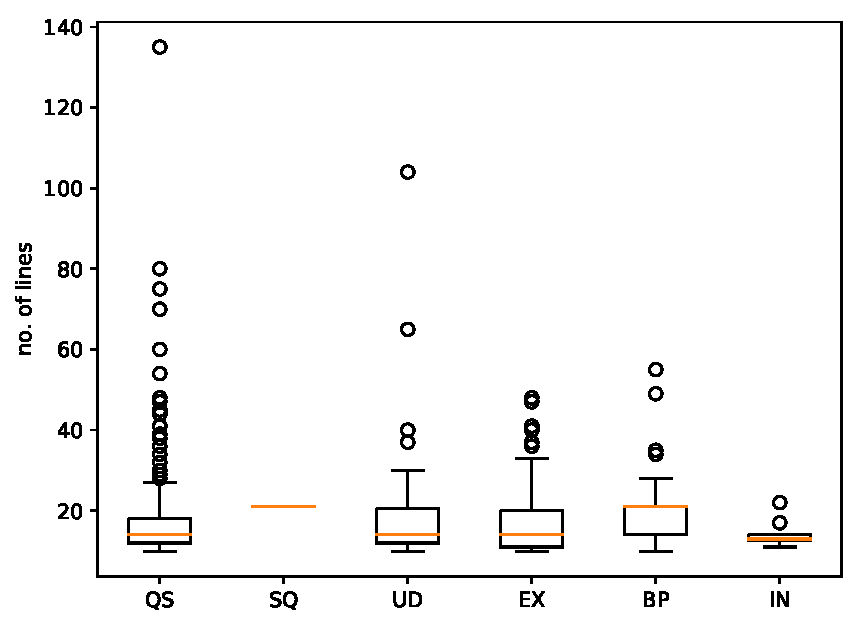
\includegraphics[width=0.5\linewidth]{../boxplot_clone_size}
	\caption{Size of online code clones.}
	\label{fig:boxplotclonesize}
\end{figure}

Regarding increasing the minimum clone size to more than 10 lines (e.g. 15 lines), we added an analysis of the clone size as shown in Figure \ref{fig:boxplotclonesize}. We found that the distribution of true clones; QS, SQ, UD, EX, BP, IN; mainly cover the size from about 10 to 20 lines. Increasing the threshold to be higher than 10 would remove some of the trivial BP and IN clone pairs which are not interesting for this study. However, it will also remove some of the true non-trivial clone pairs in QS, SQ, UD, and EX.

Regarding decreasing the minimum clone size to be less than 10 lines, we reran the two clone detection tools (Simian and SourcererCC) again using a minimum clone size of 6 lines, another well-accepted minimum clone size in clone benchmark~\citep{Bellon2007}. Simian reported 67,172 clone candidate pairs and SourcererCC reported 7,752 clone candidate pairs with 776 common clone pairs using Bellon's ok-match threshold $t=0.5$. With this large amount of clone candidate pairs, it is not feasible to manually confirm all of the clones and we must rely on sampling. Moreover, it is known that lowering the number of minimum clone lines is harmful to precision. This will result in weaker findings and weaker conclusion. Thus, we decide to retain the minimum clone size of 10 lines to keep the balance between the number of non-trivial clone pairs and the feasibility of manual clone investigation.

We have modified the paper to include this discussion in RQ2.

\rcomment{
 A similar concern exists on page 5, where t=0.7 is chosen. Sure, it worked in another context, but did they show that a 0.7 threshold is OK to use for SO snippets? I think you can also vary this t value and examine its impact.
}

We selected the Bellon's ok-match threshold of 0.7 because it is a standard value in clone benchmarking \citep{Bellon2007} and also used in other study of clones, e.g.~\cite{Sajnani2016}. Nevertheless, we agree that varying the threshold ($t$) value is beneficial to the validity of the findings so we did an analysis by choosing five $t$ values of 0.1, 0.3, 0.5, 0.7, and 0.9 and studied the clone candidates. As shown in the our paper, by setting $t=0.7$ according to Bellon's study, we found 97 ok-match pairs reported. On the other hand, setting $t$ to 0.1, 0.3, 0.5, and 0.9 resulted in 111, 110, 110, and 94 ok-matched pairs respectively. an analysis by choosing five $t$ values of 0.1, 0.3, 0.5, 0.7, and 0.9 and studied the clone candidates. As shown in the our paper, by setting $t=0.7$ according to Bellon's study, we found 97 ok-match pairs reported. On the other hand, setting $t$ to 0.1, 0.3, 0.5, and 0.9 resulted in 111, 110, 110, and 94 ok-matched pairs respectively.
Since the clone pairs of $t=0.1$ was the superset of other sets,  we manually checked all the 111 reported pairs.
We found one false positive pair and 110 true positive pairs. By raising the $t$ to 0.3 and 0.5, we got rid of the false positive pair and still retained all the 110 true positive pairs. All the clone pairs of $t=0.7$ (97) and $t=0.9$ (94) were also true positives due to being a subset of $t=0.5$. However, since there is a fewer true positive pairs reported (i.e.~generating false negatives), we ended up leaving some duplicates in the final merged clone set.

With this analysis, we can see that setting the threshold $t$ to 0.1 is too relaxed and results in having false positive ok-match pairs, while setting the $t$ to 0.7 or 0.9 is too strict and generates some false negative pairs. Thus, we decided to select the $t$ value at 0.5. This reduces the number of merged clone pairs to 2,290 pairs. All other numbers which derive from this merged clone pairs have been updated accordingly.
Since the clone pairs of $t=0.1$ was the superset of other sets,  we manually checked all the 111 reported pairs.
We found one false positive pair and 110 true positive pairs. By raising the $t$ to 0.3 and 0.5, we got rid of the false positive pair and still retained all the 110 true positive pairs. All the clone pairs of $t=0.7$ (97) and $t=0.9$ (94) were also true positives due to being a subset of $t=0.5$. However, since there is a fewer true positive pairs reported (i.e.~generating false negatives), we ended up leaving some duplicates in the final merged clone set.

With this analysis, we can see that setting the threshold $t$ to 0.1 is too relaxed and results in having false positive ok-match pairs, while setting the $t$ to 0.7 or 0.9 is too strict and generates some false negative pairs. Thus, we decided to select the $t$ value at 0.5. This reduces the number of merged clone pairs to 2,290 pairs. All other numbers which derive from this merged clone pairs have been updated accordingly.

\rcomment{
	\textbf{Question about clone patterns:} Table 4 lists all the clone patterns you considered. First, I have a major concern about the two most interesting patterns Q->S and S->Q. Especially in the case of S->Q, how can you be sure that this code actually came from SO? It could have come from any other project or from SO or another forum. Also, for Q->S, how can you be sure these snippets came from the Q projects? This is somewhat of a major concern since the rest of your paper is built on this. I would like to see a clear explanation of how we can be sure about this.
	
	\vspace{1ex}
	Now, you can say that we see code that is similar in Q and S or S and Q, but you can (almost) never say that this code comes from SO or from Q (to SO). This puts your toxic code idea into question and makes me take the results of RQs 1 and 2 with a grain of salt.
	
	\vspace{1ex}
	In fact, in the answer of RQ1, you explicitly say ``...share similar code with SO ...'', but throughout the paper, you present the work as if the code came from SO -> Q or vice versa.
}

For the QS clone pairs, we \textbf{manually confirmed with evidence} that the Stack Overflow code snippets were actually copied from Qualitas projects. This was done by the two authors reading the Stack Overflow answers containing the QS code snippets and looked for evidence such as explanation in the text or the code comments and made their decision. The two authors also compared their results and discussed until a consensus was made. Similarly, the same process was applied for the SQ clone pair. 
%For the SQ pair we discovered, we found
%evidence of cloning from Stack Overflow post ID 698283 to
%{\small\texttt{POIUtils.java}} in \textsf{jstock} project. The user
%who asked the question on Stack Overflow is an author of
%\textsf{jstock}. The question is about determining the right method to call
%among 7 overloading methods of {\small\texttt{setCellValue}} during runtime. We
%could not find evidence of copying or attribution to Stack Overflow in
%\textsf{jstock}. However, considering that the 25 lines of code of
%{\small\texttt{findMethodToInvoke}} method depicted in Figure 7 in Stack
%Overflow is very similar to the code in \textsf{jstock} including comments, it is almost certain that
%the two code snippets form a clone pair. In addition, the Stack Overflow answer was
%posted on March 30, 2009, while the code in {\small\texttt{POIUtils}} class in
%\textsf{jstock} was committed to GitHub on the next day of March 31, 2009.
In case of a doubt or not enough evidence, we always categorised the clone pairs into UD (unknown direction) instead. 

To emphasise this point, we also modified the answer of the RQ2 to be clearer. It now says \textit{``To answer RQ2, we found 2,076 manually confirmed clone pairs between 443 Stack Overflow code snippets
and 59 Qualitas proejcts.''.}

\rcomment{
	And given the types of clones you find (e.g., BP code), this can really come from anywhere (and more likely to come from things like tutorials or IDEs). Then, you report that 65\% of the closes are BP. AC is also not a clone really since even in your Table 4 you said AC is false clones - how can an Accidental *clone* be a false clone? If something is false, then it is not a clone.
}

You are correct regarding the BP clone pairs. They can really come from anywhere (we did find that some of the BP clone pairs were auto-generated code by NetBeans) and that is why we did not draw any conclusion about them. 
Moreover, thank you for pointing out the inappropriate naming for AC. We now renamed them from AC to NC (i.e.~Not Clones).

\rcomment{
I feel that the strongest part of the paper is the survey section. I really enjoyed the findings and think that the community can learn something from the outcomes of the survey (especially section 3.5.5). However, I did find the question in section 3.5.3 to be unfair somehow since there is really no mechanism in SO to notify anyone who used a code snippet. In fact, no one even knows who used a code snippet from SO.
}

%Our apologies if the writing in section 3.5.3 confuses you. 
The research question (section 3.5.3) is actually about notifying the answerers that their answers are already outdated, not notifying the users of the outdated code snippets. This notification to the answerer can be done by posting comments for that answer on Stack Overflow. For example, the answerer of the Stack Overflow question no.~10924648 posted a comment on his own answer saying that the answer is specifically for Spring 3.1. Moroever, another user posted a comment on the answer of the post no.~801935 that the code snippet is not of high quality and suggested an alternative in another post. We extended this discussion in Section 3.1.1 (RQ1). 

\rcomment{
Perhaps minor, but this issue really did not sit well with me, in the introduction, you say in RQ5 that you survey 607 participants, but later it turns out that only 201 responded. To me, this is somewhat misleading and does not sit well. I strongly encourage the authors to refactor such `marketing' statements.
}

You are right. We fixed the text in the RQ to say that we surveyed 201 participants.

\section{Reviewer 3}

\rcomment{
There is also no discussion if partial updates to the outdate code clones where posted in the same Q\&A threat (e.g., addressed by somebody else who just mentioned the necessary modifications or provided a link to the updated code fragment).  It would also have been interesting to know how old the Q\&As (clones) were, since the Qualitas code base is 4 years older then the StackOverflow snapshot. Not sure why you selected 2013 and not 2014 or 2012.
Average and mean time/date of the clone postings on stackoverflow would be interesting to see the distribution of the clone age (simple boxplot would do).
}

We are grateful for the insightful comment. We selected the 2013 snapshot of Qualitas data since it is the latest and the most complete snapshot (i.e.~having the highest number of Java projects) provided by the data set author. 

Regarding the age of cloned code on Stack Overflow, we did an analysis of clone ages as you suggested. We only chose the QS clone pairs since we could manually confirmed the direction of cloning. Moreover, we could searched for the date that the cloned version of the QS project appeared, which was not possible for UD, EX, BP, and IN clone pairs. 
We calculated the clone ages by counting the number of month difference from the dates of each Qualitas project to the date the answers were posted on Stack Overflow.
We drew a boxplot as you suggested and included the discussion of the statistics in RQ4. We found that the minimum, maximum, median, and average clone ages were 0, 64, 26.5 and 26 months respectively.  %(also summarised in the table below).

%\begin{table}[H]
%	\centering
%\begin{tabular}{lrrrrr}
%	\toprule
%	\multirow{2}{*}{Clone pattern} & \multirow{2}{*}{Amount} & \multicolumn{4}{c}{Age of clones (months)} \\ \cmidrule{3-6}
%	& & Min & Max & Avg. & Median \\
%	\midrule
%	QS & 153 & 0 & 64 & 26.5 & 26.0 \\
%	\bottomrule
%\end{tabular}
%\end{table}

From the data, we observed that, on average, it took around 2 years for the clones from Qualitas projects to appear on Stack Overflow answers. Some of the clones appeared on Stack Overflow almost at the same time as the original, while the oldest clones took around 5 years.

\rcomment{
I do believe the survey results from the StackOverflow contributors actually provides more meaningful insights then then the clone detection itself, since the responses by the contributors actually help explaining some of the results. The authors should provide further analysis and interpretation of the survey results.
}

We moved them to RQ1 to better link with the motivation. We also expanded the findings to include another survey, the Stack Overflow visitor survey, in order to understand the awareness of the developers on both sides: the answerers and the visitors (i.e.~information seekers). We asked the visitors their experience regarding outdated and license-incompatible code caused by copying and reusing code snippets from Stack Overflow. The findings are incorporated into RQ1.

\rcomment{
Overall discussion is very weak. While the authors went through a lengthy and detailed study of code clones published on StackOverflow and the survey of StackOverflow contributors, the paper lacks really a take home message. At the end there is no real evidence that either code clones are really toxic or bad (are they actually causing problems ? due to the use of clones. Just because a code fragment is outdated does not mean it is necessarily bad or causes any problems. What is the actual take home message from your study? Should we stop reusing code from StackOverflow? I do believe there is a need to dig deeper in the observed data and draw some real conclusions on how the observed results can benefit both the StackOverflow community and the source code community.
}

That is a good point. We relied on the two new analyses and added a new discussion about toxicity of outdated code in the Overall Discussion. 

First, from the answer to Reviewer 2, we analysed the intent behind the changes that made the code outdated and found that only 10 and 15 out of 100 cases were bug fixing and dead code. Besides that, the code were outdated because of evolution in the software (adding or enhancing features, refactoring, changing coding style, and data change).

Second, as previously discussed in the answer to Reviewer 1, we have performed an additional experiment to search for occurrences of the 100 outdated code snippets in 130,703 open source GitHub projects and found 102 occurrences of the outdated code. 47 were exact copy of the outdated versions, of which 12 were buggy. However, we could not establish evidence that the outdated code were cloned from Stack Overflow or somewhere else. We have reported the problem of race condition in two clone snippets found in deeplearning4j and Apache Hive to the developers.

To summarise, we empirically show from the surveys and the clone detection experiment that online code clones occur on Stack Overflow and the clones may become toxic due to outdated code and software license incompatibility. 
Nevertheless, we found only a small amount of toxic outdated code snippets in open source projects on GitHub. Besides 12 buggy and outdated code snippets found in 12 projects, the rest were non-harmful clones of the outdated code. Although other studies show that Stack Overflow code snippets may contain security vulnerabilities~\citep{Acar2016,Fischer2017} or API misuse~\citep{Zhang2018}, we found in this study that the damage caused by reusing outdated code on Stack Overflow is not high. 

On the other hand, the missing of licensing statement of online code clones on Stack Overflow can be more harmful. As shown in our study and also in the study by \cite{An2017}, some online clones on Stack Overflow are originally licensed under more restrictive license than Stack Overflow's CC BY-SA 3.0. If these missing-license online clones are reused in a software with incompatible license, the software owner may face legal issues. The software auditing service such as Black Duck Software or nexB, which can effectively check for license compliance of code copied from open source projects, cannot check for the original license of the code snippets on Stack Overflow. Although Stack Overflow answerers participated in our survey believe that most of the code snippets on Stack Overflow are too small to claim for copyright and they fall under fair-use, there is still a risk due to different legal system in each country. For example, Germany legal system does not have a concept of fair use or the number of minimum lines of code to be consider trivial, i.e.~de minimis, is also different from case to case or from country to country. 

We also updated the Actionable Items section to reflect Reviewer 1's comment.

\vspace{1cm}

\section{Conclusion}
We would like to thank the reviewers again for their comments.
We have tried our best to address every concern that has been pointed out by the reviewers. This result in inclusion of a Stack Overflow visitors' survey, an analysis of toxic code snippets in GitHub projects, analysis of different tools' and technique's parameters, a more detailed analysis of online code clones, the updated definition of toxic code snippets, the improved overall discussion section, and other minor improvements throughout the paper.
We believe this new submission has been considerably improved from the previous version due to the insightful reviews and discussions and we are looking forward to the new reviews.

% Uncomment in case references are needed
%\bibliographystyle{plain}
\bibliographystyle{spbasic}
\bibliography{references}


\end{document}
